\documentclass[12pt]{article}
\usepackage{class/sbc-template}
\usepackage{graphicx,url}
\usepackage[utf8]{inputenc}
\usepackage[brazil]{babel}
\usepackage{multirow}
\usepackage{hyperref} 
\usepackage{abntex2cite}
     
\sloppy

\title{Um estudo sobre as entradas de dados e a experiência do usuário em sistemas computacionais para a Agricultura 4.0}

\author{Diogo C. T. Batista\inst{1}, Cléber G. Corrêa\inst{1}, Letícia M. Peres\inst{2}, Roberto Pereira\inst{2}}

\address{Universidade Tecnológica Federal do Paraná (UTFPR)\\
  Cornélio Procópio -- Paraná -- Brasil
	\nextinstitute
	Universidade Federal do Paraná (UFPR)\\
	Curitiba -- Paraná -- Brasil
	\email{diogo@diogocezar.com,clebergimenez@utfpr.edu.br,\{lmperes,rpereira\}@inf.ufpr.br}
	}

\begin{document} 

\maketitle
     
\begin{resumo} 
A Agricultura 4.0 explora a utilização de tecnologias computacionais de ponta, envolvendo a Agricultura e Pecuária de Precisão, bem como a Agricultura Digital, que empregam a automação, a robótica agrícola, \textit{Big Data}, a Internet das Coisas, entre outras. A utilização dessas tecnologias busca uma produção agrícola eficiente e sustentável, possibilitando, por exemplo, a economia de água na irrigação ou de insumos na adubagem dos solos. Entretanto, o acesso aos recursos necessários para a exploração dessas tecnologias não é a realidade de grande parte do setor agrícola. Além disso, a resistência na adoção de novas tecnologias é um problema ainda em aberto. Este trabalho busca a exploração de metodologias, estudos e comprovações, por meio de experimentos, que direcionem soluções computacionais inseridas no contexto da Agricultura 4.0, com o intúito de apoiar o desenvolvimento de sistemas nesta área. Para isso, propõe-se a análise de técnicas para projetar, implementar e avaliar sistemas computacionais, de forma colaborativa e eficiente.\\

\textbf{Palavras-chave:} Agricultura 4.0; Entradas do usuário; Sistema de apoio a decisão; Smartphones.
\end{resumo}

\section{Introdução}
\label{sec:introducao}

Serão grandes os desafios relacionados à utilização de tecnologias digitais como ferramentas de apoio ao trabalho humano de forma eficiente, eficaz e justa \cite{Rose:2019}. Para isso, a humanidade apoia-se nas descobertas e comprovações de milhares de anos da comunidade científica, que proporcionam resultados relevantes, alcançados por meio da exploração das técnicas e métodos descobertos e aprimorados ao longo dos anos.

A indústria é um exemplo de como essa evolução aconteceu. Seu marco se dá com a definição da Era Artesanal, na qual, os bens e serviços eram criados por um único indivíduo: o artesão. Este era responsável por deter todo o conhecimento dos métodos e processos para a fabricação de um produto ou para a prestação de um serviço. Com a criação e o aperfeiçoamento das máquinas a vapor, estes processos puderam ser minimamente automatizados, e isso deu origem a Primeira Revolução Industrial. A Segunda Revolução Industrial, acontece com a utilização da eletricidade e principalmente dos processos que possibilitaram a implantação da produção em massa idealizadas por Henry Ford. Já a Terceira Revolução Industrial se inicia após a Segunda Guerra Mundial, com o descobrimento e a utilização da robótica e do uso de computadores para a automação das indústrias \cite{Souza:2017}.

Mais recente, muito tem se falado sobre a Quarta Revolução Industrial, que surge em 2011 na Alemanha, com a proposta de oferecer para a indústria o que há de mais moderno em automação e sistemas inteligentes, possibilitando uma série de melhorias como por exemplo: a redução dos custos, a economia de energia e o aumento da segurança. Essas e outras melhorias têm sido exploradas por meio da utilização de ferramentas e tecnologias como: \textit{Big Data}, \textit{Analytics}, Serviços de Nuvem, Impressões 3D, Segurança Cibernética, Robôs Autônomos, Internet das Coisas, Sensores sem Fio, Realidade Aumentada, Simulação, Integração Horizontal e Integração Vertical \cite{Souza:2017}.

Além da indústria, outro setor que evoluiu muito ao longo dos anos foi a agricultura. A agricultura foi fundamental para alavancar o desenvolvimento das civilizações ao longo da história, possibilitando que comunidades nômades se estabilizarem em determinadas regiões, explorando técnicas agrícolas para a produção de seu sustento. Entretanto, o cenário atual é bem diferente dos enfrentados pelas primeiras civilizações, o crescimento populacional, e a tendência das pessoas a se tornarem cada vez mais exigentes com o que é consumido, gera um grande desafio para o setor agrícola, que precisa se posicionar eficientemente para atender estas demandas. Dessa forma, novas técnicas têm sido exploradas, e estas, compõem o termo Agricultura 4.0. Estas técnicas utilizam os mesmos métodos e processos inovadores já explorados pela Indústria 4.0, incluindo: a automação, a robótica, \textit{Big Data} e Internet Das Coisas, em um contexto de Agricultura e Pecuária de Precisão e Agricultura Digital \cite{Ribeiro:2018}.

A utilização de componentes tecnológicos não é uma novidade na Agricultura, a exploração, por exemplo, de tecnologias como o \textit{Global Positioning System} (GPS), estão presentes a algum tempo na linha de produção agrícola, conhecida como Agricultura de Precisão. A Agricultura 4.0 expande as possibilidades de explorações tecnológicas, com a utilização por exemplo de: \textbf{Sensores}; que possibilitam a coleta automática de dados sobre o solo e clima; \textbf{Veículos Aéreos Não Tripulados (VANTs ou drones) ou Satélites}, que podem apresentar recursos de imagem cada vez mais avançados, auxiliando no aumento de produtividades e ajudando a reduzir danos às lavouras, visto que possibilitam o monitoramento em tempo real; \textbf{smartphones}, que proporcionam uma interface de entrada e saída de dados rápida, acessível e conhecida por usuários de dispositivos eletrônicos \cite{Shepherd:2018}.

A Agricultura 4.0, com a utilização de sistemas de apoio à decisões, pode levar à produções mais eficientes e ao consumo mais inteligente e sustentável. Entretanto, essa transição não é uma tarefa trivial. Segundo \citeonline{Rose:2019}, a utilização destas ferramentas tecnológicas devem mudar a forma como os agricultores interagem com suas plantações, com isso, cada vez menos os trabalhadores precisão colocar a ``mão na massa'', mudando a forma como sempre interagiam com seu ofício. E isso pode dificultar a adesão de novas tecnologias. A utilização das técnicas relacionadas a agricultura de precisão demonstraram certa resistência por parte dos agricultores \cite{Rose:2019}. Entretanto, o uso em larga escala de Inteligência Artificial (IA), robótica e outras inovações emergentes, tem o claro potencial de causar consequências sociais não intencionais, imprevistas e indesejadas. Por este motivo, é importante focar em uma parte fundamental para o sucesso da aplicação de novas tecnologias: o usuário.

Grande parte das tecnologias adotadas pela Agricultura 4.0 está inserida (pelo menos em algum momento) em um sistema computacional. Sabe-se que um sistema computacional é basicamente composto pela \textit{entrada de dados}, o seu \textit{processamento} e a disponibilização dos seus \textit{resultados}. As duas últimas etapas dependem da qualidade da fonte de dados, ou seja, da entrada das informações \cite{Torres:2013}.

No âmbito agrícola, por mais automatizados que possam estar os processos de obtenções dos dados, com sensores automáticos ou análise de imagens, por exemplo, há dois principais pontos que podem aumentar ainda mais a resistência à adoção das tecnologias: \textit{Indisponibilidade de Equipamentos} e \textit{Conhecimento Empírico}. No cenário atual, não são todos os agricultores que podem destinar parte do seu faturamento para a aquisição de equipamentos modernos que facilitariam a coleta de dados. Além disso, existe uma variável de grande importância que deve ser inserida na equação da Agricultura 4.0, a experiência do agricultor com a sua propriedade e a sua área de atuação. Segundo \citeonline{Rose:2019} aproximar o usuário final do processo tecnológico, pode ser uma estratégia eficiente para a adoção de novas tecnologias.

Dessa forma, o presente projeto pode contribuir com determinados \textit{Objetivos de Desenvolvimento Sustentável}, descritos pela Organização das Nações Unidas \cite{ONU:2020}. No documento da organização, são descritos 17 objetivos que buscam concretizar os direitos humanos e promover a igualdade. Para isso, tais objetivos e metas foram definidos com o intuito de estimular ações para os próximos 15 anos, em áreas de importância crucial para a humanidade e para o planeta. Dentre os objetivos, dois deles têm relação direta com este trabalho:

\begin{itemize}
	\item \textit{Objetivo 2: Fome zero e agricultura sustentável} - Aumentar a eficiência da produção agrícola é consequência direta da proposta deste trabalho. A criação de interfaces inclusivas e que consideram a experiência profissional do usuário podem proporcionar dados de entradas mais refinados, que consequentemente, podem melhorar os resultados de apoio a decisão no domínio agrícola;
	\item \textit{Objetivo 12: Consumo e produções sustentáveis} - Neste quesito, o trabalho contribui com a proposta de uma solução eficiente, acessível (utilizando um \textit{smartphone} como equipamento, por exemplo) e sem a necessidade da aquisição de novos equipamentos para integrações tecnológicas.
\end{itemize}

\section{Objetivo}
\label{sec:objetivo}

A proposta deste projeto é a exploração de metodologias, estudos e comprovações, por meio de experimentos, que direcionem soluções computacionais inseridas no contexto da Agricultura 4.0, com o intúito de apoiar o desenvolvimento de sistemas nesta área. Para isso, propõe-se a análise de técnicas para projetar, implementar e avaliar sistemas computacionais, de forma colaborativa e eficiente.

A motivação para o presente trabalho, foi construída com base na análise de uma série de problemas, ainda abertos, na comunidade agrícola detalhados na Seção \ref{subsec:problema_investigado}. Estas questões, possibilitam a exploração de diretrizes para aprimorar a relação entre a tecnologia e a comunidade agrícola. Além disso, na exploração dos trabalhos relacionados (Seção \ref{subsec:problema_investigado}), fica evidente que a maioria dos trabalhos que aborda às inovações da Agricultura 4.0 foca nas saídas de dados (visualização de informações).e/ou entradas provenientes de sensores, permitindo um processamento para o apoio a tomada de decisão na produção agrícola.

Por se tratar de um domínio muito grande, propõe-se o direcionamento dos estudos nos sub-domínios relacionados à forma de inserção dos dados nos sistemas computacionais agrícolas. Assim sendo, a proposta é aprimorar as diferentes dimensões de informações de  São poucas as explorações com relação ao refinamento das entradas de dados. \textbf{entrada de dados}, para o desenvolvimento de sistemas computacionais de suporte a decisão. 

Explorando um a forma de como isso pode ser feito, nota-se que tais informações de entrada, não precisam ser somente texto. Normalmente essas informações são coletadas com anotações e preenchimento de formulário de atributos. Propõe-se a análise e comprovação da eficiêcia de outras técnicas como: análise deimagens, discursos (reconhecimento de voz), modelos tridimensionais, vídeos e etc; bem como combinações de entradas, como imagens com anotações textuais, ou sobreposições de destaques em áreas da imagem, permitindo maior ``interação'' com as imagens e demais entradas de dados. Os vídeos podem ser utilizados para registrar uma determinada sequência de eventos, descrevendo um fenômeno; modelos tridimensionais podem proporcionar detalhes de algum elemento da cultura (por exemplo, uma planta de soja), e podem ser construídos com imagens de diferentes ângulos de um objeto alvo. Outro ponto é a utilização de dispositivos, como os \textit{smartphones}, que se tornaram populares e possuem recursos para suportar essas entradas, como câmera e microfone.

Dessa maneira, a análise deve permitir a criação de métodos de entrada de dados que levem em consideração não somente a transcrição exata do estado atual observado pelo coletor das informações, mas também os seus \textit{insigts} com base em sua experiência e observação. A análise deve considerar a necessidade dessas entradas, como forma de usar a experiência dos usuários em campo pelo sistema; o desenvolvimento das interfaces de \textit{smartphones} para essas entradas (gráficas e sintetizadores de voz); a diversidade de usuários (agricultores, técnicos agrícolas, engenheiros agrônomos); a relação dessas entradas com outras informações (imagens, temperatura, umidade, biomassa etc), provenientes de sensores, como dispositivos posicionados na plantação, imagens de satélites, veículos aéreos não tripulados, etc, podendo complementar o processamento de informações.

A análise engloba determinadas questões:
\begin{itemize}
	\item Por que informações de entrada de sistemas agrícolas provenientes dos usuários são negligenciadas? Os sensores e outros recursos suprem a necessidade?
	\item As informações de usuários especialistas poderiam auxiliar no processamento de sistemas agrícolas, combinando com as informações de sensores?
	\item As informações dos usuários poderiam reduzir o uso de sensores, que consomem energia e necessitam de manutenção, e até mesmo o processamento do sistema, que também consome recursos?
	\item Há informações, como a identificação de um inseto em uma planta com densa vegetação, que não seriam possíveis adquirir sem manusear a planta?
	\item A diversidade de usuários (agricultores, técnicos agrícolas, engenheiros agrônomos) exigiria diferentes interfaces humano-computador?
	\item A diversidade de usuários permitiria a análise das informações por diferentes pontos de vista antes do processamento por parte do sistema?
	\item Diversos tipos de informações (imagens, voz, vídeos e modelos tridimensionais, combinação desses tipos) seriam relevantes para o sistema?
	\item Qual é o impacto de diferentes tipos de informações na interação humano-computador?
	\item Qual é o impacto do uso massivo de \textit{smartphones} (energia, conexão com rede de comunicação, memória) no campo?
\end{itemize}

A \textbf{colaboração} é uma questão importante a ser abordada, pois permite que as entradas de dados sejam enriquecidas com diversas dimensões sobre um mesmo evento observado. Esse assunto é argumento na Seção \ref{sec:analise_critica_relevancia}

A \textbf{eficiência} das métricas e metodologias a serem propostas pelo trabalho, deverão passar por um processo de comprovação melhor detalhado na Seção \ref{sec:metodos_materiais}. Para isso, após definição do objeto de estudo principal do trabalho, deve-se desenvolver uma solução que aplique as métricas e diretrises identificadas como hipóteses, com o intúito de realizar a comprovação de sua eficiência e eficácia.

\section{Trabalhos Relacionados}
\label{sec:trabalhos_relacionados}

O trabalho de \citeonline{Zhai:2020} apresenta como desafios para os sistemas de apoio a decisão agrícola: a simplificação de interfaces gráficas dos usuários e utilização de conhecimento dos especialistas do domínio do sistema. Além disso, são abordadas alternativas às entradas de dados comuns, como por exemplo: a utilização do reconhecimento de voz ou a utilização gestos. Outro ponto importante está relacionado ao processo de extração das informações da fonte de dados. Modelos tridimensionais, análise de imagens ou vídeos, e imagens interativas podem ser pontos ainda a serem explorados no contexto em que este trabalho se aplica. Este tema relaciona-se com o trabalho proposto validando a necessidade do aprimoramento das interfaces utilizadas para a extração dos dados de forma eficiente e agradável.

\citeonline{Gutierrez:2019} demonstram por meio da comparação de trabalhos, que a utilização de diversas fontes de informações de entradas é um ponto desejável para a automatização e autonomia na Agricultura 4.0. As principais comparações estão relacionadas às formas de visualização de dados processados. As entradas dos dados são tratadas de forma superficial. Os autores reafirmam a preocupação do presente trabalho em inserir diversas dimensões em uma mesma fonte de dados, e que o processo de obtenção de dados refinados pode aprimorar os resultados obtidos.

Nos trabalhos de \citeonline{Walling:2020} e \citeonline{Lundstrom:2018} é mostrada a importância da participação do usuário no processo de obtenção de dados. Profissionais com a experiência de seu domínio, são capazes de enriquecer toda a cadeia de inferência nos sistemas de apoio a decisão, independente do domínio de conhecimento no qual os sistemas estão inseridos. Com esses estudos, fica claro que a participação multidisciplinar em toda a cadeia dos sistemas de apoio a decisão podem fazer uma diferença expressiva nos resultados.

O sistema AgroDSS, explorado por \citeonline{Rupnik:2019}, é um exemplo de sistema elegível às melhorias propostas por este trabalho. Nessa abordagem, a maioria dos dados coletados é baseada apenas em informações inseridas por meio de formulários de atributos textuais.

O sistema Adama Alvo é um aplicativo para dispositivo móvel com a finalidade de auxiliar na identificação de doenças, pragas e ervas daninhas em diferentes culturas. Um dos seus principais objetivos é fornecer uma base de dados \textit{offline} para o usuário, de forma que seja possível analisar e comparar em tempo real uma praga encontrada em uma folha com uma foto da mesma. Além disso, o aplicativo permite o envio de imagens por parte do usuário para serem analisadas pelos especialistas da empresa Adama, que posteriormente podem catalogá-la e disponibilizá-la no aplicativo, auxiliando outros agricultores \cite{AdamaAlvo:2020}.

Na Figura \ref{fig:adamalvo} pode-se observar a interface do sistema Adama Alvo. Pela interface gráfica do aplicativo, é possível navegar entre categorias (doenças, pragas e ervas daninhas), bem como outras informações de saída. Na demonstração, uma coleção de lagartas é exibida. Também nota-se como é possível obter os detalhes de um inseto específico (percevejo verde) e como o aplicativo oferece o apoio ao usuário mostrando a previsão do tempo.

\begin{figure}[!htb]
	\centering
  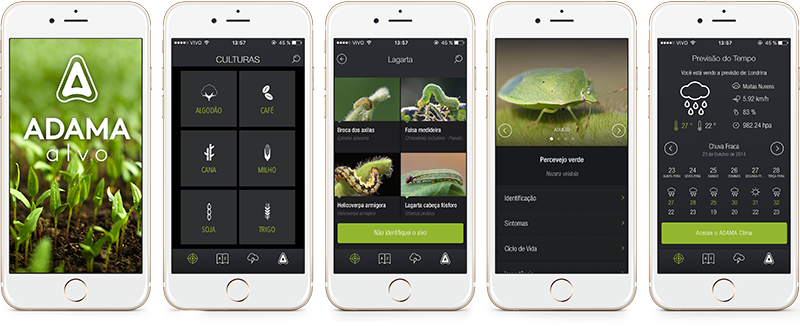
\includegraphics[scale=0.5]{images/AdamaAlvo.png}
  \caption{Interfaces gráficas do sistema Adama Alvo em diferentes situações de uso \cite{AdamaAlvo:2020}.}
  \label{fig:adamalvo}
\end{figure}

\section{Análise Crítica e Relevância}
\label{sec:analise_critica_relevancia}

No cenário agrícola, são vários os papéis dos profissionais que compõem toda a cadeia de produção. A obtenção dos dados utilizados nos sistemas computacionais de apoio à agricultura deve levar em consideração a diversidade de usuários, como agricultores, técnicos agrícolas, engenheiros agrônomos, entre outros. As experiências desses múltiplos profissionais poderiam ser utilizadas para os sistemas computacionais. Por exemplo, para uma nova praga identificada em uma folha de soja, o \textbf{agricultor} poderia inserir as informações relacionadas as suas experiências, como por exemplo se já houve alguma praga com indícios semelhantes aos encontrados, a quanto tempo, por quanto tempo, e como foi resolvido. Enquanto que o \textbf{engenheiro agrônomo} poderia inserir para esta mesma entrada informações extraídas de sua experiência em outras fazendas. Dessa forma consegue-se extrair diversas \textbf{dimensões} a partir de uma única entrada de dados \cite{Walling:2020}.

Segundo uma pesquisa divulgada pela Fundação Getúlio Vargas (FGV-SP), o Brasil tem hoje dois dispositivos digitais por habitante, incluindo \textit{smartphones}, computadores, \textit{notebooks} e \textit{tablets} \cite{FGV:2020}. Nesse sentido, o país teria aproximadamente 420 milhões de aparelhos digitais ativos. Dessa forma, fica bastante claro que estes dispositivos já fazem parte do dia a dia de muitas pessoas, inclusive dos que fazem parte de toda a cadeia agrícola.

A utilização de \textit{smartphones} e computadores propõe uma solução acessível para um dos pontos mencionados em \citeonline{Rose:2019}, que argumentam que é necessário ampliar as noções de ``inclusão'' em inovação responsável para atender às diversas formas de como os agricultores devem interagir com as fazendas inteligentes. Estes dispositivos já fazem parte da rotina de trabalho do público alvo, não sendo necessários outros investimentos ou aquisições, e ainda assim, possibilitando a inclusão desse público em novas ferramentas criadas para a Agricultura 4.0.

Como pode ser visto em \citeonline{Massruha:2017}, e nos trabalhos relacionados (Seção \ref{sec:trabalhos_relacionados}), o foco de sistemas computacionais na Agricultura 4.0 está nos resultados obtidos pelas informações fornecidas por meio das saídas desses sistemas. No cenário proposto pela Agricultura 4.0, grande parte dos trabalhos evidenciam que as informações que alimentam os sistemas, podem ser obtidas de forma automatizada, através de sensores ou pela análise de imagens, por exemplo. Entretanto, nem sempre essa é uma realidade aplicável a todos, pelo alto custo e difícil aderência. Outros sistemas, mesmo que completos em termos de sensores e outros recursos tecnológicos, utilizam ainda, entrada manual de informações por parte dos seus usuários, normalmente por meio de formulários com campos pré definidos (comumente dados no formato texto). Sensores e outros recursos também exigem monitoramento de energia, manutenção e desempenho.

\section{Problema a ser Investigado}
\label{subsec:problema_investigado}

O principal problema de pesquisa a ser tratado por este trabalho está relacionado a questões sobre como projetar, implementar e avaliar sistemas computacionais colaborativos eficientes para apoiar a tomada de decisão dos usuários no domínio da agricultura 4.0.

Os seguintes tópicos resumem em linhas gerais, quais são os problemas a serem explorados durante o desenvolvimento do projeto:

\subsection{Entrada de Dados Acessível}
\label{subsubsec:entrada_dados_acessivel}

São poucos os trabalhos encontrados na literatura que descatam a importância no processo de coleta de dados dos sistemas de apoio a decisão. Grande parte dos trabalhos, como demontrado em \cite{Massruha:2017} possuem o foco nos processos de análise e apoio a decisão. Estes trabalhos de pesquisa, normalmente, são suportados por grandes instituições (como Universidades ou empresas privadas) que provêm recursos (como sensores ou drones) para a captação de dados no desenvolvimento dos experimentos. Com tais recursos, os experimentos tendem a focar nos processos que geram os resultados e consequentemente demonstram a eficiência e a eficácia das técnicas propostas pela Agricultura 4.0. Entretanto essa não é a realidade de grande parte dos agricultores, como argumenta \cite{Rose:2019}. Os estudos propostostos por este trabalho, ajudam a resolver o problema da falta de acessibilidade aos recursos necessários para obtenção de dados, permitindo, mesmo que de uma forma menos eficiente e automatizada, a utilização de tecnologias da Agricultura 4.0 por qualquer usuário da cadeia agícola que possua apenas um \textit{smartphone}.

\subsection{Entrada Direcionada}
\label{subsubsec:entrada_direcionada}

No âmbito agrícola, é bastante comum termos grandes áreas de plantio. Mapear toda a área com dispositivos automatizados poderia gerar um custo muito grande para os agricultores, principalmente se destarcamos a necessidade de manutenção dos equipamentos que captam as informações dos campos, bem como o consumo de energia elétrica por estes dispositivos. Nesse cenário o presente trabalho também atua na pesquisa de alternativa que possibilitem envolver os fazendeiros no processo de obtenção dos dados. Isso poderia ser feito utlizando a sua experiência e conhecimento de sua propriedade para intuitivamente direcionar a coleta de dados em áreas que pudessem apresentar uma anomalia.

\subsection{Arguição dos Especialistas}
\label{subsubsec:arquicao_especialistas}

A utilização de recursos automatizados como drones ou sensores tendem a facilitar muito o processo de obtenção de dados em uma fazenda que aplica técnicas da Agricultura 4.0. Tratando de cenários nos quais essa já seja uma realidade, estes recursos automatizados normalmente apenas armazenam uma representação da realidade obtida em algum instante. Por exemplo, um sensor de humidade, poderia registrar os índices de humidade do solo a cada hora. Ou ainda, um drone, poderia fotografar uma área com baixa produtividade. Estes dados não levam em consideração alguns aspéctos que poderiam ser enriquecidos com a arguição de um especista, por exemplo um agrônomo. Por este motivo, este trabalho propõe a investigação de técnicas que possibilitem a inclusão de novas dimensões na coleta de dados, unindo por exemplo, a obtenção automática da humidade do solo com informações e experiências de um agrônomo especialista, que poderia por exemplo, informar que apesar de uma leitura de humidade ter ficado fora da expectativa, isso foi advento de uma anormalidade, por ele observada.

Para os cenários nos quais se utiliza a captação automática dos dados, boa parte das abordagens visto em \cite{Massruha:2017} fazem essa captura de forma contínua e initerruptamente, propondo abordagens que tratem grandes volumes de dados. Esta abordagem por gerar grandes custos, inserindo, por exemplo, dados muitos parecidos que não ajudam na inferência nos resultados dos sistemas de apoio a decisão. Ao utilizar tratativas com mais dimensões, criando por exemplo visões diferentes de agricultores, técnicos agrícolas ou engenheiros agrônomos sobre uma mesma entrada de dados, poderia ajudar na obtenção de dados mais refinados e consequentemente na economia de recursos para manter a coleta automatizada.

\subsection{Interações Manuais}

Quando se trata de agricultura, podemos extender a uma infinidade de procedimentos de análise em diversos tipos de cenários. Existem diversos tipos de plantações: soja, milho, café, entre outros. Cada plantação possui sua particularidade. Em cenários nos quais uma plantação apresente vegerações mais densas, entende-se como um problema a captação automática de evidências que comprovem a presença de algum tipo de praga. Essencialmente, apresença dos agricultores e fazendeiros, no dia a dia, analisando as plantações é essencial para o acompanhamento do seu processo produtivo. Uma vegetação densa, poderia esconder uma praga de uma foto aérea feita por um drone, por exemplo. No trabalho proposto, busca-se uma alternativa a este cenário, permitindo a inclusão manual destas informações que podem ser importantes para análise de inferências de apoio a decisão.

\subsection{Experiência e Interface}

A experiência do usuário com um dispositivo computacional pode influenciar diretamente na adoção de novas tecnologias ou sistemas. É bastante comum a resistência por parte de novos usuários na adoção de sistemas que ainda não tiverem contato. Como objeto de estudos deste trabalho, propõe-se ainda, descobertas relacionadas ao entendimento do perfil do público alvo, e a criação e exploração de personas, que representem os usuários e suas peculiaridades. Criando, desta forma, interfaces que possam ser objetivas, claras, atrativas e principalmente funcionais. Outro desafio a ser explorado é a interação multi-dimensional da entrada de dados, que propõe-se ser refinada, simultaneamente, por diversos colaboradores e que resultem em uma única fonte de dados, possibilitando a inferência de apoio a decisão extraídas de dados refinados e alinhados com as realidades do cenário agrícola apontado por parte da cadeia que já atua na manutenção desta propriedade.

No apêndice \ref{ape:problemas} estão listados, de forma expandandia estes e outros possíveis problemas a serem analisados.

No apêncide \ref{ape:cenario_possivel} ilustra-se um possível cenário, com a utilização de um aplicativo hipotético aplicando alguns dos conceitos a serem explorados pelo trabalho.

\section{Métodos e Materiais}
\label{sec:metodos_materiais}
		
Os métodos para a realização da pesquisa incluem:

\begin{itemize}
	\item Projeto e desenvolvimento de protótipos de sistemas computacionais (aplicativos) para validação;
	\item Planejamento, organização e execução de experimentos envolvendo usuários, normalmente com a utilização de questionários para coletar opiniões referentes as percepções desses usuários na interação humano-computador, bem como no levantamento de requisitos, para verificar a importância das informações de entrada. Informações como número de cliques, tempo de uso, também podem ser usadas na avaliação do aplicativo. No âmbito de experimentos com usuários, será realizada a submissão de projeto para avaliação de Comitê de Ética em Pesquisa com Seres Humanos da UTFPR\footnote{Disponível em: http://www.utfpr.edu.br/comissoes/permanentes/comite-de-etica-em-pesquisa} (CEP-UTFPR), utilizando a Plataforma Brasil, do Ministério da Saúde\footnote{Disponível em: http://plataformabrasil.saude.gov.br/login.jsf};
	\item Revisão da literatura, podendo utilizar métodos formais de pesquisa, como a revisão sistemática, que fornece um protocolo para o levantamento bibliográfico \cite{Kitchenham:2004};
	\item Análise de resultados utilizando testes estatísticos para verificar a significância das diferenças entre os grupos amostrais comparados (Friedman, ANOVA – Análise da Variância, t-test, Wilcoxon, Mann-Whitnney etc); e estatística descritiva (principalmente gráficos). Os testes estatísticos dependem das características dos dados (normalidade da distribuição, homogeneidade das variâncias, independência e aleatoriedade na coleta etc) e oferecem intervalos de confiança para a análise.
\end{itemize}

Métodos, técnicas e ferramentas de Engenharia de Software serão estudados para uso no trabalho, auxiliando no projeto e desenvolvimento dos protótipos.

Os materiais consistem em \textit{smartphones}, dos próprios usuários; bem como serviços de nuvem para processamento das informações adicionadas pelos usuários. Uma avaliação da aquisição de determinados sensores para medição de informações, tais como temperatura e umidade do solo, será realizada. Adicionalmente, informações de terceiros podem ser empregadas, tais como imagens de satélites e de sítios eletrônicos sobre o clima. 		

A cultura foco provavelmente será a de soja, devido a parceria da UTFPR com a Empresa Brasileira de Pesquisa Agropecuária (Embrapa), situada em Londrina, que trabalha principalmente com a produção da soja. A Embrapa é uma empresa pública de pesquisa vinculada ao Ministério da Agricultura, Pecuária e Abastecimento do Brasil. O seu principal objetivo é a viabilização de soluções provenientes de pesquisas, além do desenvolvimento para a sustentabilidade da agricultura em benefício da sociedade brasileira. A parceria atualmente visa o desenvolvimento de dois sistemas:

\begin{itemize}
	\item Sistema para identificação de pragas, doenças e plantas daninhas da cultura de soja, com suporte \textit{web} e dispositivos móveis. A utilização de imagens capturadas pelos usuários é um dos requisitos do sistema;

	\item Sistema para acompanhamento do crescimento da planta de soja, apresentando os estádios fenológicos, com suporte \textit{web} e dispositivos móveis. A utilização de modelos tridimensionais e vídeos para saída de informações ou visualização por parte dos usuários está prevista. Exemplo de alguns estádios fenológicos da soja podem ser observados na Figura \ref{fig:estadios_fenelogicos}.
\end{itemize}

\begin{figure}
	\centering
  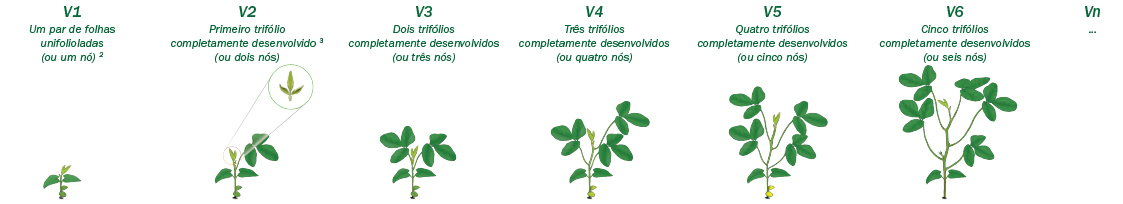
\includegraphics[scale=0.5]{images/EstadiosFenologicos.png}
  \caption{Alguns dos estádios fenológicos da planta da soja (Embrapa).}
  \label{fig:estadios_fenelogicos}
\end{figure} 

Esses sistemas ou módulos desses sistemas poderão ser empregados em estudos de caso, servindo como protótipos para validação, se necessários. 

\section{Plano de Trabalho e Cronograma}
\label{sec:plano_trabalho_cronograma}

O plano de trabalho é composto pelas seguintes atividades principais, dispostas no cronograma apresentado na Tabela \ref{tab:cronograma}, separadas por quadrimestres de cada ano:

\begin{enumerate}
	\item Obtenção de créditos, cursando disciplinas;
	\item Estudo de métodos para mapeamento ou revisão sistemática, permitindo o levantamento de trabalhos na literatura, bem como métodos, técnicas e ferramentas da Engenharia de Software para o desenvolvimento de protótipos;
	\item Estudo do estado da arte, considerando sistemas computacionais para dispositivos móveis voltados para a agricultura 4.0 e seus usuários;
	\item Levantamento de requisitos, especialmente funcionalidades relacionadas as entradas de dados dos usuários;
	\item Exame de proficiência de língua estrangeira;
	\item Exame de qualificação;
	\item Especificação de um sistema computacional para dispositivos móveis, indicando a arquitetura do sistema e principais desafios no desenvolvimento;
	\item Implementação de protótipo para validação;
	\item Elaboração de documentação para Comitê de Ética em Pesquisa com Seres Humanos da UTFPR;
	\item Testes envolvendo usuários;
	\item Redação de artigos científicos a serem submetidos aos principais eventos e periódicos da área de interesse;
	\item Redação da tese;
	\item Defesa.
\end{enumerate}

As atividades e os períodos serão ajustados conforme o edital do Programa de Pós-Graduação em Informática da UFPR.

\begin{table}[htbp]
	\centering
	\begin{tabular}{|c|c|c|c|c|c|c|c|c|c|c|c|c|}
	\hline
	\multirow{2}{*}{AT} & \multicolumn{3}{c|}{\textbf{Ano 1}} & \multicolumn{3}{c|}{\textbf{Ano 2}} & \multicolumn{3}{c|}{\textbf{Ano 3}} & \multicolumn{3}{c|}{\textbf{Ano 4}} \\ \cline{2-13} 
											& Q1         & Q2         & Q3        & Q1         & Q2         & Q3        & Q1         & Q2         & Q3        & Q1         & Q2         & Q3        \\ \hline
	1                   & •          & •          & •         &            &            &           &            &            &           &            &            &           \\ \hline
	2                   &            &            &           & •          &            &           &            &            &           &            &            &           \\ \hline
	3                   &            &            &           & •          & •          & •         & •          &            &           &            &            &           \\ \hline
	4                   &            &            &           &            & •          &           &            &            &           &            &            &           \\ \hline
	5                   &            &            &           &            & •          &           &            &            &           &            &            &           \\ \hline
	6                   &            &            &           &            & •          &           &            &            &           &            &            &           \\ \hline
	7                   &            &            &           &            & •          &           &            &            &           &            &            &           \\ \hline
	8                   &            &            &           &            &            & •         & •          & •          &           &            &            &           \\ \hline
	9                   &            &            &           &            &            &           &            &            & •         &            &            &           \\ \hline
	10                  &            &            &           &            &            &           &            &            &           & •          &            &           \\ \hline
	11                  &            &            &           &            &            & •         & •          & •          & •         & •          & •          & •         \\ \hline
	12                  &            &            &           &            &            &           &            &            & •         & •          & •          & •         \\ \hline
	13                  &            &            &           &            &            &           &            &            &           &            &            & •         \\ \hline
	\end{tabular}
	\caption{Cronograma de Execução das Atividades}
	\label{tab:cronograma}
\end{table}

Com o objetivo de manter a constante comunicação, e principalmente o acompanhamento e direcionamento das atividades, reuniões semanais devem ser realizadas. Estas reuniões podem ser realizadas de forma presencial (quando possível) ou por meio de vídeo chamadas.

\section{Resultados Esperados}
\label{sec:resultados_esperados}

Pretende-se com a análise das entradas de informações dos usuários, verificar a importância e o impacto dessas informações nos sistemas computacionais para a Agricultura 4.0, permitindo o desenvolvimento de sistemas para uma produção agrícola eficiente e sustentável. Conforme a literatura, há um maior interesse nas saídas de informações para os usuários em sistemas computacionais para a agricultura, especialmente nos sistemas de apoio a tomada de decisão. Outros tipos de informações, como imagens, voz, modelos tridimensionais e vídeos, inseridos pelos usuários em campo por meio de \textit{smartphones}, podem ser explorados, além das entradas baseadas em textos e devido a popularização e recursos desses dispositivos.

Espera-se, por fim, a submissão de artigos para conferências e periódicos científicos da área de Ciência da Computação para publicação, como o \textit{ACM Computing Surveys}, \textit{Computer Graphics and Applications}, \textit{Journal on Interactive Systems}, \textit{Computers and Electronics in Agriculture}, \textit{Symposium on Applied Computing}, Simpósio Brasileiro de Engenharia de Software.

\bibliographystyle{sbc}
\bibliography{pre-project}

\appendix

\section{Problemas de Pesquisa}
\label{ape:problemas}

A seguir lista-se características de sistemas colaborativos (gerais e específicos), relacionadas entre sí, e seus possíveis problemas:

\begin{itemize}
	\item \textbf{atualização em tempo real} - Problemas: múltiplos acessos simultâneos; necessidade de exibição de alertas e erros sobre atrasos; regras de funcionamento (entrada, processamento e saída);
	\item \textbf{múltiplos dispositivos para entrada e saída de dados} - Por exemplo: smartphones, desktops, sensores e robôs. Problemas: integração; interoperabilidade; escalabilidade de dispositivos; tolerância a falhas - possibilidade de substituição de sensores danificados;
	\item \textbf{múltiplos usuários} - Por exemplo: agricultores, técnicos agrícolas, engenheiros agrônomos. Problemas: usabilidade (facilidade de uso, segurança, satisfação, acessibilidade, memorização do usuário), envolvendo interfaces humano-computador e formas de interação; definição de grupos de usuários; carga cognitiva (muitas tecnologias e formas de uso); escalabilidade de usuários; regras de uso; atribuição de significado e interpretação das informações;
	\item \textbf{múltiplas plataformas das fontes de entrada} - Por exemplo: diveras plataformas de smartphones. Problemas: integração; interoperabilidade; usabilidade (facilidade de uso, segurança, satisfação, acessibilidade, memorização do usuário), envolvendo interfaces humano-computador e formas de interação;
	\item \textbf{múltiplos tipos de informações de entrada} - Por exemplo: imagens, voz, texto e vídeos. Problemas: armazenamento e processamento (imagens podem ocupar mais espaço), usabilidade (facilidade de uso, segurança, satisfação, acessibilidade, memorização), envolvendo interfaces humano-computador e formas de interação; carga cognitiva (muitas tecnologias e formas de uso;
	\item \textbf{múltiplos tipos de informações de saída} - Por exemplo: imagens, áudio, texto, modelos tridimensionais e vídeos. Problemas: armazenamento e processamento, usabilidade (facilidade de uso, segurança, satisfação, acessibilidade, memorização), envolvendo interfaces humano-computador e formas de interação; carga cognitiva (muitas tecnologias e formas de uso);
	\item \textbf{múltiplas informações sobre o domínio} - Por exemplo: planta, clima, pragas, ervas daninhas, doenças. Problemas: especificação de subdomínios; granularidade (sistema incorpora informações em atualizações); relação dos subdomínios – planta e clima, planta, pragas e clima);
	\item \textbf{informações de entradas de múltiplos usuários} - Por exemplo: agricultores, técnicos agrícolas, engenheiros agrônomos. Problemas: problemas de conexão com a Internet em regiões afastadas; de consumo de energia; de prioridade dependendo do nível do usuário e do nível de grupo de usuários do mesmo nível; de necessidade de diferentes interfaces humano-computador e formas de interação; de necessidade de definição de níveis e grupos; de processamento e armazenamento local, envolvendo o que pode ser processado e armazenado localmente de acordo com os recursos de hardware e software, o consumo de energia, de maneira a não prejudicar a entrada de novas informações
	\item \textbf{informações de saídas para múltiplos usuários} - Por exemplo: agricultores, técnicos agrícolas, engenheiros agrônomos. Problemas: de usabilidade (facilidade de uso, segurança, satisfação, acessibilidade, memorização), preferências dos usuários, envolvendo interfaces humano-computador e formas de interação);
	\item \textbf{informações de entradas de múltiplos sensores e robôs} - Problemas: conexão com a Internet em regiões afastadas; de nível de autonomia; de consumo de energia; de processamento e armazenamento local, envolvendo o que pode ser processado e armazenado localmente de acordo com os recursos de hardware e software, o consumo de energia, de maneira a não prejudicar a entrada de novas informações)
	\item \textbf{priorização das informações do domínio} - Por exemplo: o processamento de determinadas informações tem prioridade. Por exemplo, uma atividade de colheita está em andamento e o processamento de informações sobre o clima tem prioridade sobre o processamento de informações sobre pragas, no entanto, pode-se perder inferências. Problemas: necessidade da participação de usuários para definição de prioridades; da inviabilidade devido a quantidade de informações e necessidade de agrupamento (clusters) de informações por data, região, clima, tipo da informação, fonte, ou combinação (região e clima); flexibilidade na combinação de informações)
	\item \textbf{sincronização das informações de entrada na nuvem (cloud computing), que  envolve:}
		\begin{itemize}
			\item \textbf{priorização da informação a ser processada: a mesma informação é recebida pelo servidor ao mesmo tempo de diferentes fontes} - Por exemplo: do sensor A e do usuário 1. Problemas: identificação das similaridades; definição de prioridades com a participação de usuários;
			\item \textbf{complementação da informação: a mesma informação é recebida pelo servidor ao mesmo tempo de diferentes fontes} - Exemplo: sensor A e do usuário 1), mas de diferentes tipos (texto, imagem e voz), e elementos podem ser extraídos para completar ou confirmar a informação. Problemas: identificação das diferenças, extração e complemento; custo/benefício da  confirmação em termos de processamento, recursos utilizados;
			\item \textbf{completude da informação} - Por exemplo: a informação é recebida pelo servidor, mas incompleta, como por exemplo, uma imagem incompleta. Problemas: identificação das lacunas e correção, por aproximação, interpolação, utilização de um outro tipo de informação, adoção de um padrão, emissão de avsios para usuários sobre a necessidade de completar a informação – dependência de conexão com a Internet, energia, processamento; custo/benefício de cada forma de completude)
			\item \textbf{informação adicional automática} - Por exemplo: uma informação adicional é adicionada automaticamente em uma informação capturada pelo usuário. Por exemplo, o usuário captura uma imagem usando o smartphone, e o sistema busca automaticamente a geolocalização e o clima. Problemas: conexão com a Internet em regiões afastadas; de consumo de energia; de processamento e armazenamento local, envolvendo o que pode ser processado e armazenado localmente de acordo com os recursos de hardware e software, o consumo de energia, de maneira a não prejudicar a entrada de novas informações);
			\item \textbf{classificação da informação após o processamento} - Por exemplo: informação foi útil, parcialmente útil ou inútil, atribuindo nível de qualidade para a informação. Problemas: custo/benefício para a classificação; de necessidade da participação de usuários; da inviabilidade devido a quantidade de informações e necessidade de agrupamento (clusters) de informações por data, região, clima, tipo da informação, fonte, ou combinação (região e clima); flexibilidade na combinação de informações);
		\end{itemize}
\end{itemize}

\section{Cenário Possível}
\label{ape:cenario_possivel}

Para ilustrar as possibilidades a serem exploradas, descreve-se a utilização de um aplicativo em um cenário hipotético, no qual:

\begin{enumerate}
	\item Um fazendeiro, motivado pelo desconhecimento de uma praga, captura uma imagem de um inseto em uma planta de soja usando seu \textit{smartphone};
	\item A imagem pode receber informações adicionais no próprio \textit{smartphone}, tais como: anotações da quantidade, nome do inseto, enfatizando o tamanho do inseto e o estádio fenológico da planta;
	\item Ainda na imagem, pode ser possível a inclusão de anotações ou destaques em pontos que pudessem ser circulados, pelo fazendeiro, demonstrando pontos de atenção que pudessem ser analisados;
	\item Um engenheiro agrônomo, parceiro deste fazendeiro, analisa a mesma imagem em seu próprio perfil do aplicativo, de forma remota, inserindo e/ou complementando informações sobre o cenário investigado;
	\item Todas as imagens poderiam servir de fonte de dados: a original, a com as anotações do fazendeiro e do engenheiro agrônomo;
	\item Por conta de uma possível dificuldade de conexão (muito comum no cenário rural) o envio das informações poderia não acontecer imediatamente. Mas a operação pode ser marcada como sucesso, deixando essa atividade uma fila de execução em \textit{background};
	\item O próprio sistema registra as coordenadas de geolocalização bem como o momento (horário/dia) desta captura ou oferece a possibilidade de inserção manual destas informações (prevendo a instabilidade da conexão);
	\item Ao receber as informações, um sistema computacional em nuvem, pode relacionar as imagens recebidas com uma ou mais imagens aéreas, capturadas por veículos aéreos não tripulados da mesma região onde está a planta, ou regiões adjacentes em um ou mais momentos anteriores, buscando por insetos. O sistema computacional pode registrar dia e horário de captura da imagem, de modificação, de envio com sucesso;
	\item O sistema computacional pode ainda utilizar utilizar bases de informações compartilhadas entre diferentes regiões e usuários aumentando o refinamento na inferência das informações de apoio a decisão.
\end{enumerate}

\end{document}